\section*{Appendix A: IUBH TOR Specification}
\addcontentsline{toc}{section}{Appendix A: IUBH TOR Specification}
\subsection*{Problem and solution}

Students enrolled to distance learning courses at IUBH have access to a website within the university’s “CARE portal” that allows them to get an overview of the current state of booked modules and the grades they got for them. However, at the time of writing, there is no notification system in place that would let them know about a new grade, which leads for thousands of students to the tedious task of continually logging in to the “CARE portal” and navigating to that website, often multiple times a day. 

IUBH TOR is addressing this problem by providing fast and instant access to all information regarding students courses. Like their current status, grades, and other data provided by the CARE system. It will furthermore regularly check for updates and notify users about changes made to their transcripts of records, so they do not have to check manually.

\subsection*{Functional requirements}

\subsubsection*{App Startup}

As a student, I want to get presented the login dialog when I am currently not signed in (yet), so I can provide my credentials and sign in.

As a student, I want to get presented the course list dialog when I am currently signed in, so I can start using the app directly.

\subsubsection*{Dialog: Login}

As a student, I want to be able to sign in to the app so I can use its features.

\begin{itemize}
\item The dialog provides a text field for my user name, a password field, and a submit button (M01).
\item The button is only enabled when both the user name and the password are being provided.
\item User name and password count as provided when both contain at least one character.
\item When the authentication succeeds, I am being forwarded to the course list.
\item When the authentication fails, an error message is shown (M02).
\end{itemize}

\subsubsection*{Dialog: Course List}

As a student, I want to be able to sign out directly from the course list dialog, so I can make sure the app stops pulling data from CARE or sign in with another account.

As a student, I expect all my data to be deleted from the storage of the app after I signed out, so I can be sure there is no personal data left.

As a student, I expect data to be fetched from CARE immediately after I signed in to the app so I can see the latest data.

As a student, I want to be able to fetch new data from CARE through „pull to refresh” at any given time so I can manually check for updates.

As a student, I expect a loading indicator and some information text to appear while data is being fetched from CARE so I can see and understand what is happening (M03).

As a student, I expect any error that occurred while loading data to result in a visible error message whenever I started the process personally, or it got started automatically after signing in, so I can make a decision based on that error message (M04).

As a newly enrolled student, I expect some information being shown that there is no data available to display yet instead of an empty screen when there‘s no course to display for my account, so I don‘t confuse that state with an erroneous behavior of the app (M05).

As a student, I want to see all the courses I had or will have an exam for in a list (M06), including course name, exam date, exam status, and grade (if passed).

As a student, I want to see when the data from CARE has been updated for the last time, so I can decide on whether I should try to refresh myself or not.

As a student, I want to navigate to a course's detail dialog by selecting its entry in the list of all courses, so I can see all the detailed information that is not shown on the list.

\subsubsection*{Dialog: Course Detail}

As a student, I want to see detailed information about a course on its detail page so I can see all the things that is not shown on the list (M07).

\subsubsection*{Background Synchronization and Notification}

As a student, I want the app to check regularly for updates to my transcript of records and to notify me when something has changed, so I can stay up to date.

As a student, I want a system notification to be shown when something changed at my transcript of records so I can get notified about that change (M08).

\subsection*{Mockups}

\begin{figure}[H]
\center
\begin{tabular}{c@{\hskip 1in}c}
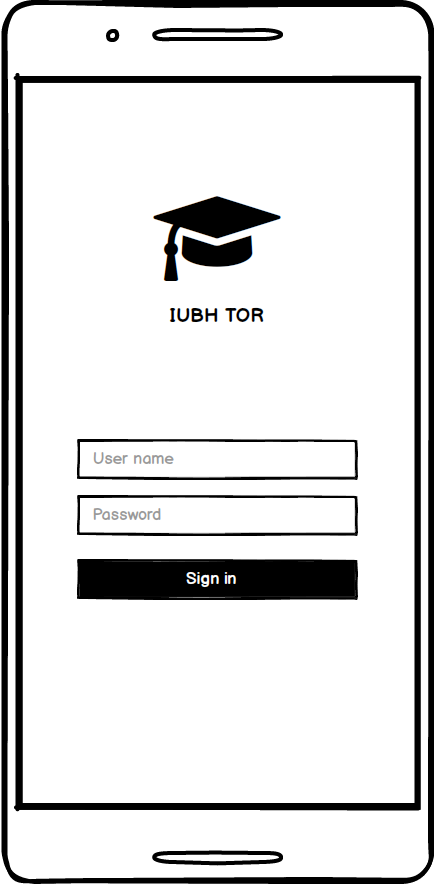
\includegraphics[width=55mm]{m01} & 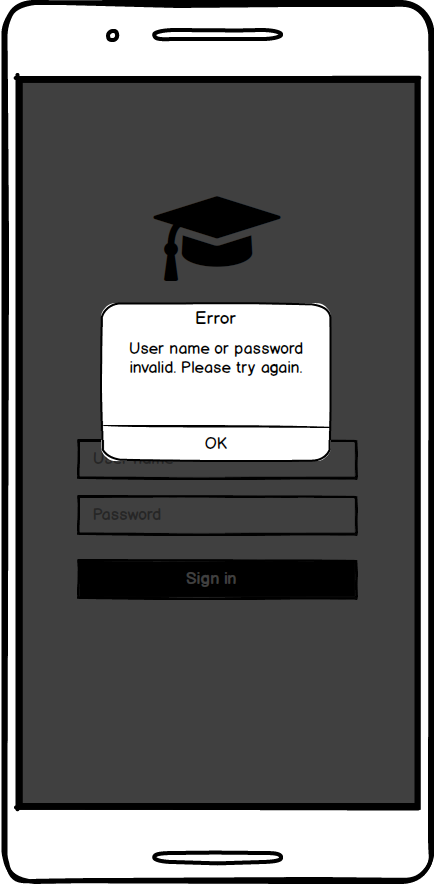
\includegraphics[width=55mm]{m02} \\
M01 & M02 \\[25pt]
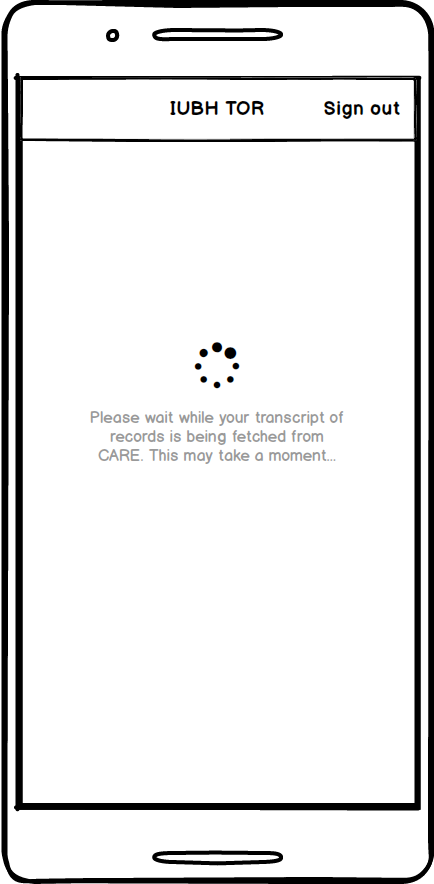
\includegraphics[width=55mm]{m03} &  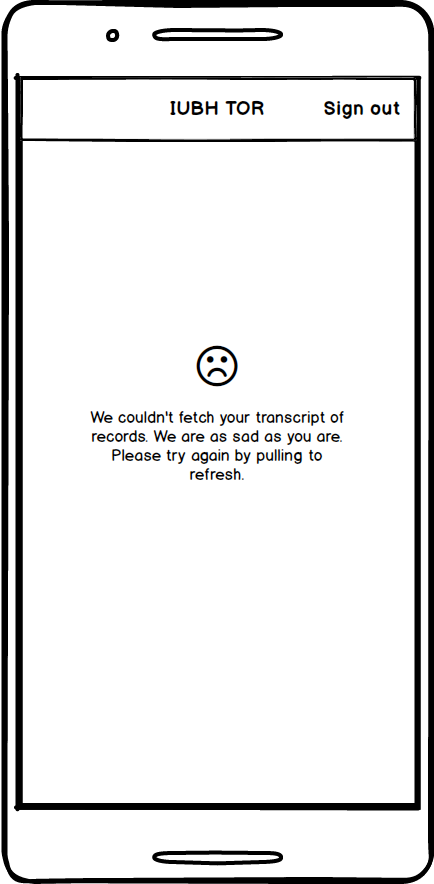
\includegraphics[width=55mm]{m04} \\
M03 & M04 \\
\end{tabular}
\end{figure}
\vfill

\begin{figure}[H]
\center
\begin{tabular}{c@{\hskip 1in}c}
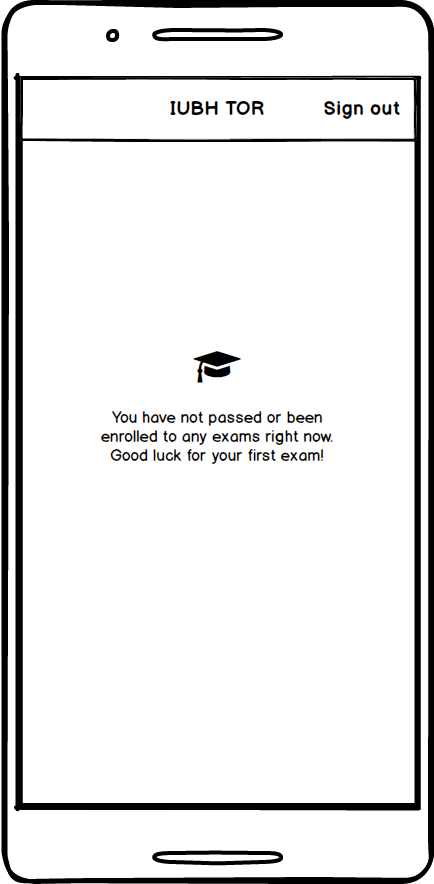
\includegraphics[width=55mm]{m05} & 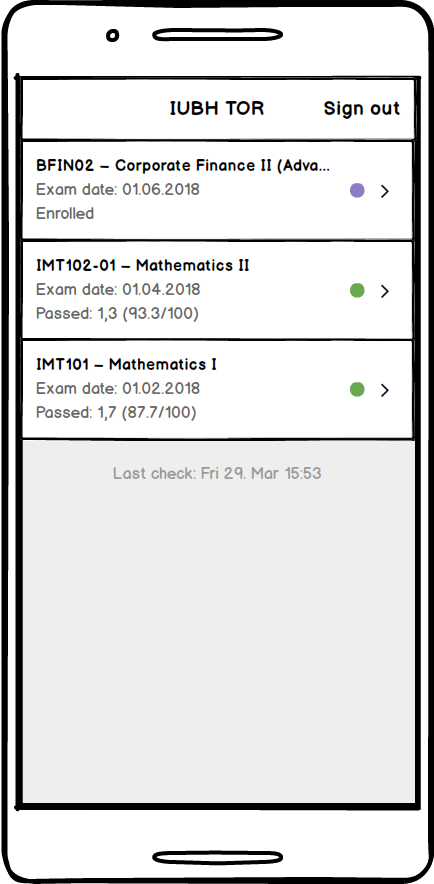
\includegraphics[width=55mm]{m06} \\
M05 & M06 \\[25pt]
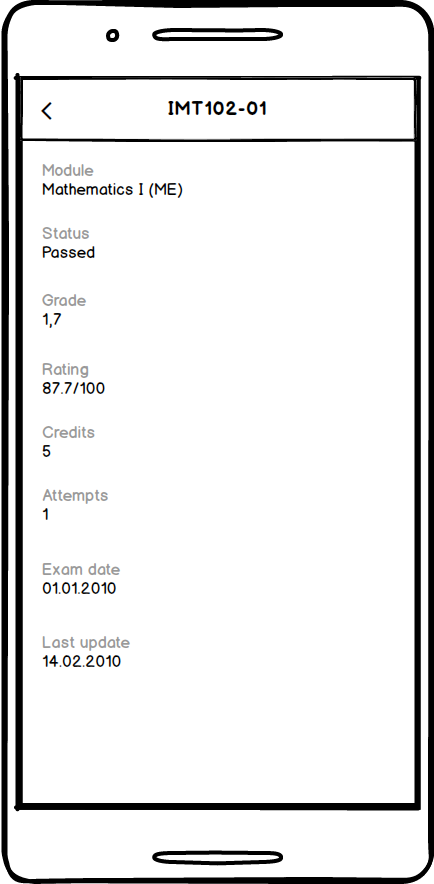
\includegraphics[width=55mm]{m07} &  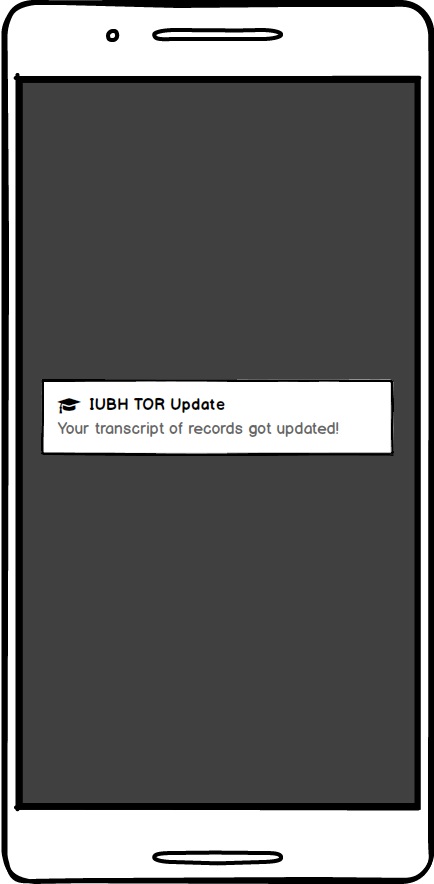
\includegraphics[width=55mm]{m08} \\
M07 & M08 \\
\end{tabular}
\end{figure}

